 
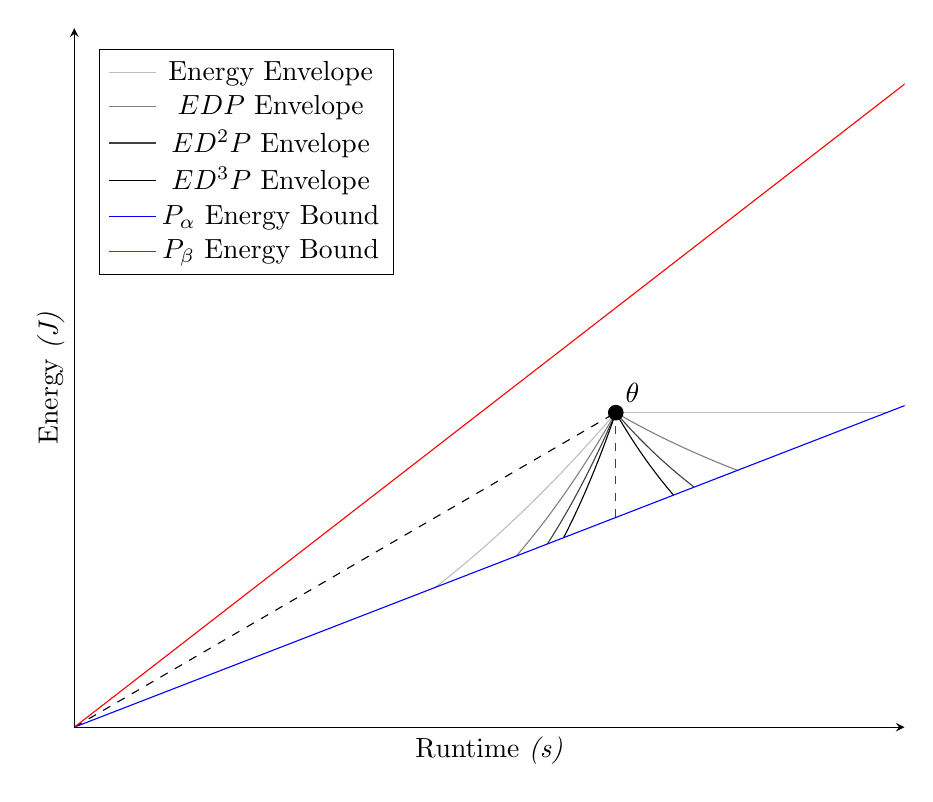
\begin{tikzpicture}
  \begin{axis}[ticks = none, 
    axis x line=bottom,axis y line=left,
    ylabel={Energy \emph{(J)}}, xlabel={Runtime \emph{(s)}}, axis on top,
    ymin=0, ymax=3000,
    xmin=0, xmax=46,
    width=\linewidth,
    legend style={legend pos=north west}
    ]

    %% Model Parameters %%
    \pgfmathsetmacro{\baselinepower}{30} % NOP code
    \pgfmathsetmacro{\rooflinepower}{60}
    \pgfmathsetmacro{\codepower}{(\baselinepower + \rooflinepower) / 2}
    \pgfmathsetmacro{\codetime}{30}
    % Sadly, pgfplots sucks too much to calculate cube roots
    \pgfmathsetmacro{\anodex}{26.20741}
    \pgfmathsetmacro{\anodey}{\anodex * \baselinepower}
    \pgfmathsetmacro{\cnodex}{34.34143}
    \pgfmathsetmacro{\cnodey}{\cnodex * \baselinepower}
    \pgfmathsetmacro{\tnodex}{27.25681}
 
    %% Intermezzo Values %%
    \pgfmathsetmacro{\codeenergy}{\codepower * \codetime}
    \pgfmathsetmacro{\baselineenergy}{\baselinepower * \codetime}
    \pgfmathsetmacro{\rooflineenergy}{\rooflinepower * \codetime}
    \pgfmathsetmacro{\lowdisplayline}{(2 * \baselinepower + \codepower) / 3}
    \pgfmathsetmacro{\highdisplayline}{(1 * \rooflinepower + 1 * \codepower) / 2}

    % arguments: code power, code time, x, n 
    \pgfmathdeclarefunction{optimizationbound}{4}{%
      \pgfmathparse{((#1 * #2^(#4 + 1)) / #3^#4)}%
    }
    \pgfmathdeclarefunction{definitionbound}{4}{%
      \pgfmathparse{((#1 / #2^(#4 + 1)) * #3^(#4 + 2))}%
    }
 
    % Constant Time and Power Dashes
    \draw[darkgray, dashed] ({axis cs:\codetime,\baselineenergy}) -- ({axis cs:\codetime,\codeenergy});
    \draw[dashed] ({axis cs:0,0}) -- ({axis cs:\codetime,\codeenergy});

    \pgfmathsetmacro{\dzerodefnx}{20}
    \pgfmathsetmacro{\dzerooptx}{45}
    \addplot[domain=\dzerodefnx:\codetime, lightgray] { definitionbound(\codepower, \codetime, x, 0};
    \addplot[domain=\codetime:\dzerooptx, lightgray, forget plot] { optimizationbound(\codepower, \codetime, x, 0)};
    \addlegendentry{Energy Envelope}

    \pgfmathsetmacro{\donedefnx}{24.4948974278}
    \pgfmathsetmacro{\doneoptx}{36.742346141747674}
    \addplot[domain=\donedefnx:\codetime, gray] { definitionbound(\codepower, \codetime, x, 1};
    \addplot[domain=\codetime:\doneoptx, gray, forget plot] { optimizationbound(\codepower, \codetime, x, 1)};
    \addlegendentry{$EDP$ Envelope}

    \pgfmathsetmacro{\dtwodefnx}{26.2074139421}
    \pgfmathsetmacro{\dtwooptx}{34.34142727659995}
    \addplot[domain=\dtwodefnx:\codetime, darkgray] { definitionbound(\codepower, \codetime, x, 2};
    \addplot[domain=\codetime:\dtwooptx, darkgray, forget plot] { optimizationbound(\codepower, \codetime, x, 2)};
    \addlegendentry{$ED^2P$ Envelope}

    \pgfmathsetmacro{\dthreedefnx}{27.1080601083}
    \pgfmathsetmacro{\dthreeoptx}{33.200457591009645}
    \addplot[domain=\dthreedefnx:\codetime, black] { definitionbound(\codepower, \codetime, x, 3};
   
    \addlegendentry{$ED^3P$ Envelope}
 \addplot[domain=\codetime:\dthreeoptx, black, forget plot] { optimizationbound(\codepower, \codetime, x, 3)};

    % ALPHA BASELINE BOUND 
    \addplot[domain=0:50, blue] {\baselinepower * x};
    \addlegendentry{$P_{\alpha}$ Energy Bound} 
    % BETA ROOFLINE BOUND
    \addplot[domain=0:50, red] {\rooflinepower * x};
    \addlegendentry{$P_{\beta}$ Energy Bound} 



    \node[circle,fill,inner sep=2pt] at (axis cs:\codetime,\codeenergy) {};
    \node[above right] at (axis cs:\codetime,\codeenergy) {$\theta$};

 \end{axis}
\end{tikzpicture}
